\documentclass[a4paper]{article}
\usepackage[utf8]{inputenc}
\usepackage[english]{babel}
\usepackage{amsmath} % per ambienti tipo cases
\usepackage{amssymb}
\usepackage{mathtools}
\usepackage{siunitx}
\usepackage{graphicx} % per includere figure
%\usepackage{subfigure}
\usepackage{booktabs} % per le tabelle
\usepackage{caption}
\usepackage{fancyhdr}
\usepackage{hyperref}
\usepackage[section]{placeins}
\usepackage{microtype}
\usepackage{caption}
\usepackage{subcaption}
\captionsetup[subfigure]{labelfont=rm}
\usepackage{verbatim} %multiline comments
%\usepackage[backend=biber, style=numeric, safeinputenc, sorting=none]{biblatex}
%\addbibresource{source.bib}	% uncomment for bibliography



%opening
\title{}
\author{}

\pagestyle{fancy}
\lhead{Musical Acoustics}
\chead{HL1}
\rhead{10743504, 10751919}
\newcommand{\Rarrow}{\mbox{\Large$\Rightarrow$}}

\begin{document}

\begin{titlepage}	
	\newcommand{\HRule}{\rule{\linewidth}{0.5mm}} % Defines a new command for horizontal lines, change thickness here
	
	\center % Centre everything on the page
	
	%------------------------------------------------
	%	Headings
	%------------------------------------------------
	
	
\includegraphics[width=.4\textwidth]{Logo_Politecnico_Milano.png}\\[0.4cm]
	\textsc{\LARGE}\\[0.3cm] % Main heading such as the name of your university/college
	
	\textsc{\large MSc. Music and Acoustic Engineering}\\[1cm] % Minor heading such as course title
	
	\textsc{\Large Musical Acoustics - A.Y. 2020/2021}\\[0.5cm] % Major heading such as course name
	
	%------------------------------------------------
	%	Title
	%------------------------------------------------
	
	\HRule\\[0.4cm]
	
	{\huge\bfseries H4 - Impedance maxima of a compound horn }\\[0.4cm] % Title of your document
	
	\HRule\\[1.5cm]
	
	
	
	{\large\textit{Authors' IDs:}}\\
	10743504, 10751919, % Your name
	%\\ \textsc{Gruppo 11}
	
	%------------------------------------------------
	%	Date
	%------------------------------------------------
	
	\vfill\vfill\vfill % Position the date 3/4 down the remaining page
	
	{\large\today} % Date, change the \today to a set date if you want to be precise
	
	%------------------------------------------------
	%	Logo
	%------------------------------------------------
	
	\vfill\vfill
	%\includegraphics[width=0.2\textwidth]{Politecnico_di_Milano.eps}\\[1cm] % Include a department/university logo - this will require the graphicx package
	
	%----------------------------------------------------------------------------------------
	
	\vfill % Push the date up 1/4 of the remaining page
	
	
\end{titlepage}

\section{Impedance maxima of the pipe}

\begin{figure}[h!]
	\centering
	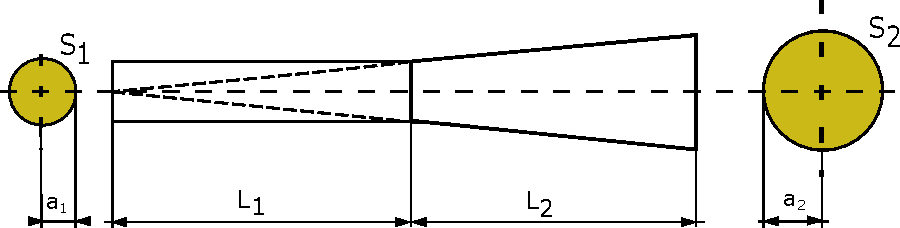
\includegraphics[width=0.8\linewidth]{diagramma.pdf}
	\caption{Scheme of the compound horn system. Beside each end a drawing of the corresponding cross section can be seen.}
	\label{fig:diag}
\end{figure}

In order to compute the acoustic input impedance of a pipe, one needs to account not only for the air contained in the pipe as an ideal fluid but also for two phenomena occurring around it: the radiation load at the end and the wall losses along its length. The latter is relevant for narrow pipes in particular, but in our case, since the ratio between the pipe's length and the radius of its cross section is $L_1/a_1 = 10$, it is clear that we are not dealing with this condition. Moreover, a common way to characterize the influence of the viscous drag is the ratio of the pipe radius with the boundary layer thickness $r_v$. If this parameter is greater than $10$, it is usually considered safe to neglect the wall losses. Since $r_v \propto \sqrt{f} $, this might not be true at low frequencies; however, in our case, we can see that $r_v$ increases very rapidly from zero and at $\SI{1}{\hertz}$ is already $ \sim 30 $. We assume, therefore, that it is safe for us to ignore such losses in the computation of the impedance. 

Concerning the radiation, instead, we know that its influence on an open-ended pipe is usually not negligible. At low frequency, the strategy that is commonly used to address the study of radiation is to add an end correction $\Delta^{open}$ . At first order in $ka$ the radiation impedance of an open end is equal to the input impedance of an open pipe of length $\Delta^{open}$. We take the value $\Delta^{open} = 0.61 a$; this holds well under the assumption $ka \ll 1 $. However, for us $ka = 1$ at $\sim 1$ kHz, which is well inside the range of frequencies we are interested in. At higher frequencies it is still possible to use this model\footnote{As long as the wavefronts are planar, i. e. for $ka<3.83$.}, but the end correction decreases with $ka$. This means that the values for the frequencies of the impedance maxima we will compute will be slightly underestimated in the higher range.

The input impedance of the pipe is therefore, in our model:

\begin{align*}
	Z_{in} = jZ_0 \tan{kL} \qquad & \text{, with } L = L_2 + \Delta^{open} = L_2 + 0.61a_1
\end{align*}

The corresponding maxima are at
$$ f_n = \biggl(n - \frac{1}{2}\biggr) \frac{c}{2L}, \qquad n \in \mathbb{N} $$

\section{Compound horn}
We know that the expression for the input impedance of the pipe in terms of the load impedance $Z_L$ at the far end is
\begin{equation}\label{eq:zin}
	Z_{in} = Z_0 \frac{Z_L \cos{kL_2} + jZ_0\sin{kL_2}}{jZ_L \sin{kL_2} + Z_0 \cos{kL_2}}
\end{equation}
with $Z_0 = \frac{\rho c}{S_1}$ being the characteristic impedance of the pipe. Characterizing the frequency-domain acoustic behavior of the compound system, therefore, is just a matter of writing the input impedance of the horn. Once again, this is quite straightforward for a conical horn terminating in an ideal open end:
\begin{equation}\label{eq:zc}
	Z_c = \frac{j\rho c}{S_1} \biggl( \cot{kL_1} + \frac{1}{kx_1} \biggr)^{-1}
\end{equation}

However, if we want to include the radiation impedance, we run into the same problem as before, except even worse, since the radius of the open end of the horn is double that of the pipe. In this case we get $ka = 1$ at $\sim 545$ Hz: as we will see shortly, the first maxima and minima of the impedance do not surpass this value by a large margin, so we can assume that using a constant value of the end correction doesn't have a devastating impact on our estimation of their position. When considering higher frequencies, this won't be true anymore.

With that being said, let us now discuss the maxima and minima of the impedance at low frequencies. For the impedance of the horn we can take (\ref{eq:zc}) and substitute $L_1$ with $L_1 + 0.61a_2 $. We can then use this value of $Z_c$ in lieu of the impedance load $Z_L$ in (\ref{eq:zin}). This gives us an equation for the maxima and one for the minima: the former is obtained by requesting that the denominator in (\ref{eq:zin}) be zero, while the latter results from doing the same thing with the numerator. Explicitly:

\begin{align*}
	&\text{\underline{maxima}:} \quad & \tan{kL_2} - \cot{kL_1} + \frac{1}{kx_1} = 0\\
	&\text{\underline{minima}:} \quad & \cot{kL_2} + \cot{kL_1} + \frac{1}{kx_1} = 0
\end{align*}

The results are shown together with a graph of the magnitude of the impedance in Fig. \ref{fig:maxmin}.

\begin{figure}[h!]
	\centering
	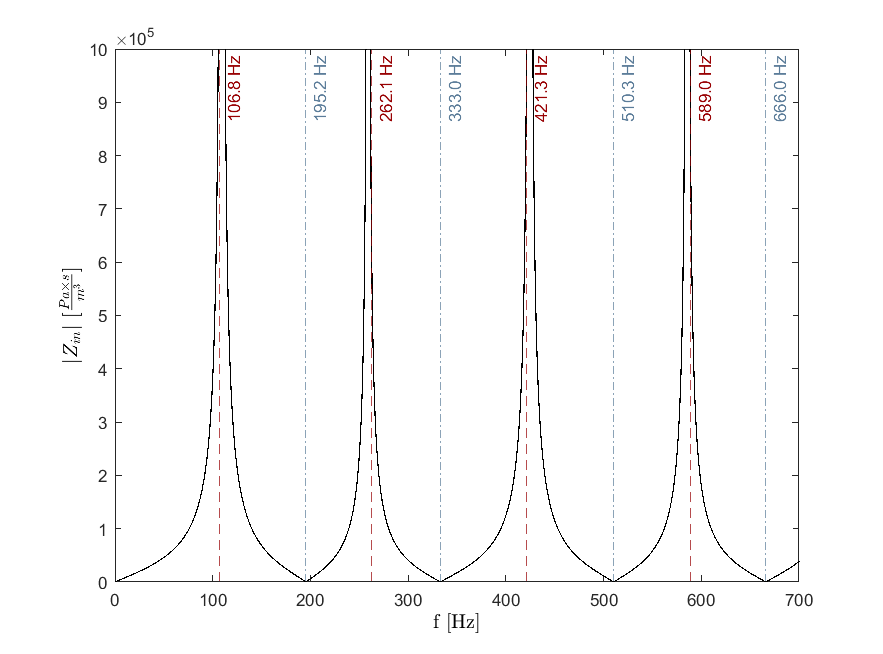
\includegraphics[width=0.8\linewidth]{maxmin.png}
	\caption{Magnitude of the impedance of the compound horn. The red vertical lines correspond to the maxima, while the blue ones to the minima.}
	\label{fig:maxmin}
\end{figure}



\end{document}